%!TeX root=../carlo_master.tex
\chapter{Experimental analysis: binary classification}\label{sec:binary_experiments}

This chapter evaluates the decision strategies of Chapter~\ref{sec:binary} on fourteen datasets, ten base classifiers, and ten objectives (five cost matrices and five non-decomposable maximization metrics; see Section~\ref{sec:binary_objectives}). The cost-blind plug-in rule is suboptimal in nearly every regime considered, and two routes recover competitive performance: post-hoc calibration composed with the analytical Elkan threshold, and cross-validated empirical optimization of the threshold (EmpiricalCV). EmpiricalCV wins or ties the per-row best strategy on $87\%$ of cost cells and $99.9\%$ of maximization-metric cells. Post-hoc calibration composed with the analytical rule is the highest-rate strategy among the non-tuning options on miscalibrated non-neural estimators under decomposable cost objectives.

\section{Experimental setup}

We use a standardized protocol that holds the data partition, preprocessing, and base estimator fixed across decision strategies for a given dataset.

\subsection{Datasets}
The benchmark draws fourteen binary datasets from OpenML \citep{vanschoren2014openml}, selected along four axes. First, size spread: the three sample-size tiers (small with $N < 10^3$; medium, $10^3 \leq N < 10^4$; large, $N \geq 10^4$) vary the budget available to the strategies that consume a held-out partition (calibrator fits and the empirical threshold search), so the comparison is exercised from tens of positives in the validation split up to tens of thousands. Second, imbalance diversity: prevalence ratios span $1.0$ (\textit{madelon}) to $42.0$ (\textit{mammography}), with coverage at every order of magnitude in between, so the cost-asymmetric objectives can be exercised under both near-balanced and high-skew regimes. Third, overlap with prior cost-sensitive learning benchmarks: \textit{sonar}, \textit{pima\_diabetes}, and \textit{german\_credit} appear in \citet{sheng2006thresholding}, and \textit{adult} is used in \citet{elkan2001foundations}, so part of the pool is directly comparable to earlier results. Fourth, task difficulty: the pool spans easy problems on which the base classifiers reach near-ceiling discrimination and harder ones on which every estimator in the benchmark remains well below ceiling, so the decision strategies are evaluated on top of probability estimates of widely varying quality. Table~\ref{tab:dataset-summary-binary} lists the per-dataset sample sizes, feature counts, and class prevalences.

\begin{table}[H]
  \centering
  \caption{Summary of binary classification datasets used in the experiments. Superscripts denote OpenML dataset IDs. Numerical and Categorical are the counts of raw numerical and categorical input features; Encoded is the model input dimensionality after one-hot encoding of the categorical features. The imbalance ratio (IR) is the size of the majority class divided by that of the minority class.}%
  \label{tab:dataset-summary-binary}
  \resizebox{\textwidth}{!}{%
  \begin{tabular}{lrrrrl}
\toprule
 &  & \multicolumn{3}{c}{Features} &  \\
\cmidrule(lr){3-5}
Dataset & Samples & Numerical & Categorical & Encoded & IR \\
\midrule
sonar\textsuperscript{\tiny 40}~\citep{gorman1988sonar} & 208 & 60 & 0 & 60 & 1.1 \\
ionosphere\textsuperscript{\tiny 59}~\citep{sigillito1989ionosphere} & 351 & 34 & 0 & 34 & 1.8 \\
wdbc\textsuperscript{\tiny 1510}~\citep{street1993wdbc} & 569 & 30 & 0 & 30 & 1.7 \\
pima\_diabetes\textsuperscript{\tiny 37}~\citep{smith1988diabetes} & 768 & 8 & 0 & 8 & 1.9 \\
german\_credit\textsuperscript{\tiny 31}~\citep{hofmann1994germancredit} & 1000 & 7 & 13 & 61 & 2.3 \\
pc3\textsuperscript{\tiny 1050}~\citep{sayyadshirabad2005promise} & 1563 & 37 & 0 & 37 & 8.8 \\
ozone\textsuperscript{\tiny 1487}~\citep{zhang2008ozone} & 2534 & 72 & 0 & 72 & 14.8 \\
madelon\textsuperscript{\tiny 1485}~\citep{guyon2004madelon} & 2600 & 500 & 0 & 500 & 1.0 \\
spambase\textsuperscript{\tiny 44}~\citep{hopkins1999spambase} & 4601 & 57 & 0 & 57 & 1.5 \\
phoneme\textsuperscript{\tiny 1489}~\citep{elena1993phoneme} & 5404 & 5 & 0 & 5 & 2.4 \\
jm1\textsuperscript{\tiny 1053}~\citep{sayyadshirabad2005promise} & 10885 & 21 & 0 & 21 & 4.2 \\
mammography\textsuperscript{\tiny 310}~\citep{woods1993mammography} & 11183 & 6 & 0 & 6 & 42.0 \\
bank\_marketing\textsuperscript{\tiny 1461}~\citep{moro2011bank} & 45211 & 7 & 9 & 51 & 7.5 \\
adult\textsuperscript{\tiny 1590}~\citep{kohavi1996adult} & 48842 & 6 & 8 & 105 & 3.2 \\
\bottomrule
\end{tabular}
  }
\end{table}


Preprocessing is applied via a \texttt{scikit-learn} \citep{pedregosa2011scikit} \texttt{ColumnTransformer} fitted once on the full dataset prior to splitting: numerical features are median-imputed and standardized; categorical features are most-frequent-imputed and one-hot encoded. Fitting the transformer on the full dataset, rather than refitting it inside each split, introduces a small amount of information leakage from the test partition into the imputation, standardization, and one-hot category statistics. This is a deliberate simplification: the same fitted transformer is reused across all strategies and splits for a given dataset, so any leakage affects all decision strategies equally and does not bias the comparison this benchmark is designed to support.

\subsection{Estimator architectures}
Ten base classifiers span a range of inductive biases and calibration profiles. The short label in parentheses after each full name is the form used as the column header in the result tables and figures of this chapter and the companion supplement:
\begin{itemize}
    \item Logistic Regression (LogReg) \citep[Ch.~4.4]{hastie2009elements}: parametric linear baseline; smooth monotonic probabilities.
    \item Gaussian Naive Bayes (GaussNB) \citep[Ch.~6.6.3]{hastie2009elements}: generative historical baseline with class-conditional Gaussian features and feature independence.
    \item LightGBM (LGBM) \citep{ke2017lightgbm}, XGBoost (XGB) \citep{chen2016xgboost}, CatBoost \citep{prokhorenkova2018catboost}: gradient-boosted trees, the standard top-performing family on tabular benchmarks in prediction quality and training and inference speed; typically discriminative but overconfident.
    \item Random Forest (RF) \citep{breiman2001random}, Extra Trees (ET) \citep{geurts2006extratrees}: bagged ensembles; averaging smooths the probability outputs and produces calibration profiles distinct from boosted trees.
    \item TabM \citep{gorishniy2025tabm}: deep tabular architecture; an MLP ensemble over shared representations.
    \item TabPFN \citep{hollmann2025accurate}, TabICL \citep{qu2025tabicl}: transformer-based in-context predictors for tabular data, evaluated only on datasets within their supported regime ($\le 10{,}000$ samples and $\le 2{,}000$ features for TabPFN\@; $\le 10{,}000$ samples and $\le 500$ features for TabICLv2, matching its tested envelope) and skipped on larger datasets.
\end{itemize}
All classifiers use default hyperparameters. The benchmark sweeps the base estimator architecture as one factor in the design but does not tune hyperparameters within each architecture, since the contribution under study is the analysis of decision strategy on top of a given estimator.

\subsection{Objectives}\label{sec:binary_objectives}
The objective set covers ten targets: five cost matrices and five maximization metrics. The cost matrices are
\begin{itemize}
    \item Symmetric: $0/1$ loss ($C_{ij} = 0$ if $i = j$, else $1$).
    \item Asymmetric $10\times$ / Asymmetric $100\times$: $C_{10} = 1$ and $C_{01} \in \{10, 100\}$ on the off-diagonals (with $C_{00} = C_{11} = 0$), so a false positive costs ten or one hundred false negatives.
    \item Non-Zero Diagonal: a matrix $C = \bigl[\begin{smallmatrix} 0.8 & 2.0 \\ 1.0 & 0.5 \end{smallmatrix}\bigr]$ with non-zero entries on the diagonal as well as the off-diagonal, so even correct predictions carry baseline loss; mixes asymmetric error costs with non-uniform correct-prediction costs.
    \item Balanced Error: the prior-weighted cost matrix $C_{00} = C_{11} = 0$, $C_{01} = 1/(2\pi_0)$, $C_{10} = 1/(2\pi_1)$, where $\pi_y = \mathbb{P}(Y = y)$ is the marginal class prior; misclassifying a class-$y$ example carries weight $1/(2\pi_y)$, so the rare class is over-weighted in inverse proportion to its frequency.
\end{itemize}
The five maximization metrics are $F_1$, $F_{0.5}$, $F_2$ (\texttt{sklearn.metrics.fbeta\_score}), MCC (\texttt{sklearn.metrics.matthews\_corrcoef}), and G-Mean (the geometric mean of per-class true-positive rates, \texttt{imblearn.metrics.geometric\_mean\_score}). These five are \emph{non-decomposable} performance measures in the sense of \citet{narasimhan2015optimizing}: each is a non-linear function of the confusion-matrix counts $(\mathrm{TP}, \mathrm{FP}, \mathrm{FN}, \mathrm{TN})$ as a whole and cannot be written as a per-sample average of a fixed loss $\tfrac{1}{n}\sum_i C_{y_i, \hat y_i}$ for any cost matrix $C$; consequently no fixed prior-weighted plug-in threshold of the calibrated $\hat p$ is Bayes-optimal across distributions, and the empirical-tuning family is the only one that targets these objectives directly.

\subsection{Decision strategies}
For each (dataset, model, objective) triple we evaluate twelve strategies that map the probability estimate $\hat{p}(x)$ to a discrete class. The strategies fall into three families: uncalibrated baselines that do not consume any held-out data, calibrate-then-decide pipelines that fit a probability transformation on a validation split before applying a closed-form threshold, and direct decision optimization that selects the threshold by minimizing empirical risk.

\paragraph{Uncalibrated baselines.} Two strategies apply a fixed threshold without consuming any held-out data: Argmax ($\tau{=}0.5$) is the cost-blind argmax rule, and Analytical ($\tau{=}p^*$) is the \citet{elkan2001foundations} threshold from Eq.~\ref{eq:elkan_threshold} applied directly to uncalibrated outputs.

\paragraph{Calibrate-then-decide.} A post-hoc calibrator is fitted to the raw probabilities on the validation set, then the analytical threshold $p^*$ or the default $\tau{=}0.5$ is applied to the recalibrated scores. Four calibrators paired with two threshold choices yield eight strategies:
\begin{itemize}
    \item Isotonic Regression (non-parametric, monotone) $\times$ \{Argmax, Analytical\}.
    \item Platt Scaling (sigmoid fit on the classifier's raw score $s(x)$, taken as the \texttt{decision\_function} output when the estimator exposes one, following scikit-learn's convention, and the raw probability $\hat p(x)$ otherwise) $\times$ \{Argmax, Analytical\}.
    \item Temperature Scaling (single-parameter logit rescaling) $\times$ \{Argmax, Analytical\}.
    \item Dirichlet Calibration \citep{kull2019beyond} $\times$ \{Argmax, Analytical\}.
\end{itemize}

\paragraph{Direct decision optimization.}
\begin{itemize}
    \item Empirical ($\tau_{\mathrm{emp}}$): exact grid search over a uniform grid of $G = 301$ thresholds on $[0,1]$, evaluated on the held-out validation set, following the algorithm of Section~\ref{sec:threshold_grid_search}.
    \item EmpiricalCV\@: same grid search, but the threshold is selected by $5$-fold stratified cross-validation on the full training set, eliminating the dedicated validation split, following Section~\ref{sec:cv_threshold}.
\end{itemize}

\subsection{Evaluation protocol}
Each dataset is split stratified $80/20$ into a training pool (\emph{train-full}) and a held-out \emph{test set}. The training pool is further split into a $70\%$ \emph{training split} and a $10\%$ \emph{validation split} relative to the full dataset.

The data budget consumed by each strategy depends on whether tuning requires a held-out signal. Argmax and Analytical use no tuning and fit the base estimator on the full $80\%$ train-full pool. The calibrate-then-decide pipelines and Empirical fit the estimator on the $70\%$ training split and tune the decision layer (calibrator parameters or threshold) on the $10\%$ validation split. EmpiricalCV fits and tunes jointly via $5$-fold stratified cross-validation over the full $80\%$ pool, matching the estimator's data budget to that of Argmax and Analytical.

The reported metric is the objective value (average cost or target metric) computed on the held-out test set, averaged over $10$ independent seeds that resample the data partition; each base estimator's own \texttt{random\_state} is held fixed across seeds, so the reported variance reflects partition resampling alone.

\section{Results and discussion}

Table~\ref{tab:model-auc-binary} reports the held-out test ROC AUC of each base estimator, computed on the positive class and averaged over the ten seeds.

\begin{table}[H]
    \centering
    \footnotesize
    \caption{Held-out test ROC AUC of each base estimator trained on the full 80\% training pool (positive class) for the binary datasets, reported as mean $\pm$ 1 SE over the ten seeds. Models skipped by a documented sample-size, feature-count, or class-count gate have no entry. Bold marks every model within 1 SE of the per-dataset best.}%
    \label{tab:model-auc-binary}
    \adjustbox{max width=\linewidth}{%
    \begin{tabular}{lcccccccccc}
    \toprule
    Dataset & LGBM & LogReg & XGB & CatBoost & RF & ET & GaussNB & TabM & TabPFN & TabICL \\
    \midrule
    sonar & 0.941 ± 0.013 & 0.853 ± 0.020 & 0.917 ± 0.012 & \textbf{0.959 ± 0.010} & 0.926 ± 0.014 & \textbf{0.969 ± 0.007} & 0.796 ± 0.019 & 0.946 ± 0.012 & \textbf{0.970 ± 0.007} & — \\
    ionosphere & 0.969 ± 0.006 & 0.897 ± 0.008 & 0.962 ± 0.006 & 0.971 ± 0.006 & 0.975 ± 0.006 & \textbf{0.985 ± 0.003} & 0.928 ± 0.006 & \textbf{0.982 ± 0.005} & \textbf{0.984 ± 0.004} & — \\
    wdbc & 0.992 ± 0.002 & 0.993 ± 0.002 & 0.993 ± 0.002 & 0.993 ± 0.002 & 0.989 ± 0.003 & 0.992 ± 0.002 & 0.984 ± 0.004 & \textbf{0.993 ± 0.002} & \textbf{0.996 ± 0.001} & \textbf{0.996 ± 0.002} \\
    pima\_diabetes & 0.811 ± 0.010 & \textbf{0.843 ± 0.011} & 0.805 ± 0.010 & \textbf{0.840 ± 0.010} & 0.830 ± 0.008 & 0.825 ± 0.009 & 0.824 ± 0.015 & 0.787 ± 0.009 & \textbf{0.853 ± 0.011} & \textbf{0.847 ± 0.011} \\
    german\_credit & 0.769 ± 0.009 & \textbf{0.781 ± 0.011} & 0.772 ± 0.009 & \textbf{0.797 ± 0.012} & \textbf{0.782 ± 0.012} & 0.770 ± 0.010 & 0.731 ± 0.008 & 0.771 ± 0.009 & \textbf{0.793 ± 0.012} & \textbf{0.791 ± 0.011} \\
    pc3 & 0.820 ± 0.005 & 0.795 ± 0.013 & 0.809 ± 0.007 & 0.833 ± 0.007 & 0.830 ± 0.010 & 0.835 ± 0.010 & 0.722 ± 0.021 & 0.804 ± 0.007 & 0.839 ± 0.008 & \textbf{0.857 ± 0.007} \\
    ozone & 0.923 ± 0.006 & 0.921 ± 0.006 & 0.919 ± 0.007 & \textbf{0.929 ± 0.007} & 0.913 ± 0.007 & 0.921 ± 0.009 & 0.839 ± 0.007 & 0.923 ± 0.009 & \textbf{0.939 ± 0.008} & \textbf{0.941 ± 0.007} \\
    madelon & 0.888 ± 0.005 & 0.569 ± 0.008 & 0.877 ± 0.006 & 0.921 ± 0.004 & 0.767 ± 0.009 & 0.720 ± 0.008 & 0.638 ± 0.008 & 0.647 ± 0.007 & 0.966 ± 0.003 & \textbf{0.972 ± 0.002} \\
    spambase & 0.989 ± 0.001 & 0.971 ± 0.001 & 0.987 ± 0.001 & 0.988 ± 0.001 & 0.986 ± 0.001 & 0.986 ± 0.001 & 0.924 ± 0.008 & 0.982 ± 0.001 & \textbf{0.992 ± 0.001} & \textbf{0.992 ± 0.001} \\
    phoneme & 0.956 ± 0.002 & 0.814 ± 0.003 & 0.956 ± 0.002 & 0.955 ± 0.002 & 0.964 ± 0.002 & 0.970 ± 0.002 & 0.816 ± 0.003 & 0.956 ± 0.002 & 0.969 ± 0.002 & \textbf{0.977 ± 0.001} \\
    jm1 & 0.745 ± 0.004 & 0.713 ± 0.004 & 0.729 ± 0.004 & 0.746 ± 0.004 & 0.751 ± 0.004 & 0.752 ± 0.004 & 0.688 ± 0.003 & 0.728 ± 0.005 & 0.762 ± 0.004 & \textbf{0.783 ± 0.003} \\
    mammography & 0.943 ± 0.009 & 0.912 ± 0.009 & 0.942 ± 0.008 & \textbf{0.960 ± 0.007} & 0.944 ± 0.010 & 0.946 ± 0.009 & 0.919 ± 0.006 & \textbf{0.953 ± 0.008} & \textbf{0.961 ± 0.006} & \textbf{0.960 ± 0.007} \\
    bank\_marketing & \textbf{0.935 ± 0.001} & 0.905 ± 0.001 & 0.931 ± 0.001 & \textbf{0.937 ± 0.001} & 0.927 ± 0.001 & 0.908 ± 0.001 & 0.807 ± 0.002 & 0.925 ± 0.001 & — & — \\
    adult & \textbf{0.929 ± 0.001} & 0.906 ± 0.001 & \textbf{0.929 ± 0.001} & \textbf{0.930 ± 0.001} & 0.902 ± 0.001 & 0.878 ± 0.001 & 0.826 ± 0.006 & 0.904 ± 0.001 & — & — \\
    \bottomrule
\end{tabular}
    }
\end{table}


Across the (dataset, model, objective) triples in the campaign, EmpiricalCV wins or ties the per-row best strategy on $87\%$ of cost cells and $99.9\%$ of maximization-metric cells.

Per-dataset means $\pm\,1$ standard error (SE) over the ten seeds for every (model, objective, strategy) combination are reported in the companion supplement (\texttt{tex/supplement/supplement.pdf} in the source repository), with cells whose mean$\,\pm\,$SE interval overlaps the best strategy's bolded. The aggregates cover all ten base classifiers.

\subsection{Calibration quality and the analytical rule}

The plug-in Analytical threshold matches direct search when the cost matrix is symmetric and separates from it as the asymmetry grows. Pooled across the ten estimators, Analytical, Empirical, and EmpiricalCV agree to within sampling error on the Symmetric and Non-Zero Diagonal matrices. On Asymmetric $10\times$ and Asymmetric $100\times$ the analytical rule trails the empirical strategies, with the per-row win-or-tie rate of EmpiricalCV larger than Analytical's on those two matrices.

The bare analytical threshold stays close to the per-row best on the three deep tabular models (TabM, TabPFN, TabICL) but trails on the seven non-neural classifiers. As the cost ratio $C_{01}/C_{10}$ departs from $1$ (Section~\ref{sec:analytical_threshold}), the Bayes-optimal threshold moves away from the bulk of the score distribution, so any systematic miscalibration of $\hat{p}(x)$ translates into a larger decision-level penalty; the deep tabular probabilities are calibrated well enough that the Elkan threshold of Eq.~\ref{eq:elkan_threshold} remains close to optimal without post-hoc adjustment, while the non-neural defaults are not. The per-classifier breakdown of Figure~\ref{fig:win-counts-binary-cost} shows the same pattern at the win-or-tie level.

Figure~\ref{fig:ci-mammography-non-zero_diagonal_cost} shows a representative cell, \textit{mammography} with TabICL under Non-Zero Diagonal: EmpiricalCV and Analytical share the lead within sampling error, the calibrate-then-Analytical pipelines form a middle band, and the cost-blind strategies trail.

% Auto-generated by experiments.analysis.generate_ci_plots --- do not edit.
\begin{figure}[H]
\centering
\adjustbox{max width=\textwidth}{%
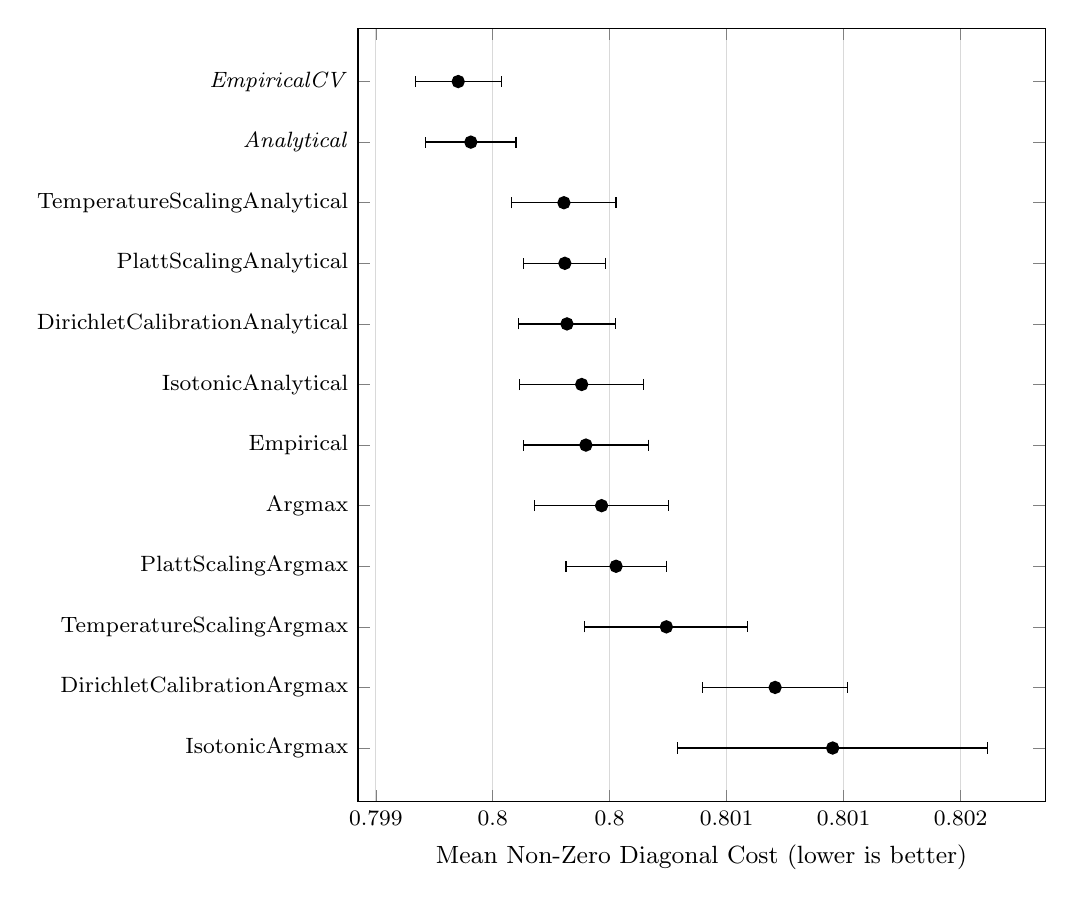
\begin{tikzpicture}
\begin{axis}[
    width=0.85\textwidth, height=11.40cm,
    xlabel={Mean Non-Zero Diagonal Cost (lower is better)},
    symbolic y coords={{EmpiricalCV},{Analytical},{TemperatureScalingAnalytical},{PlattScalingAnalytical},{DirichletCalibrationAnalytical},{IsotonicAnalytical},{Empirical},{Argmax},{PlattScalingArgmax},{TemperatureScalingArgmax},{DirichletCalibrationArgmax},{IsotonicArgmax}},
    ytick={{EmpiricalCV},{Analytical},{TemperatureScalingAnalytical},{PlattScalingAnalytical},{DirichletCalibrationAnalytical},{IsotonicAnalytical},{Empirical},{Argmax},{PlattScalingArgmax},{TemperatureScalingArgmax},{DirichletCalibrationArgmax},{IsotonicArgmax}},
    yticklabels={\textit{EmpiricalCV},\textit{Analytical},TemperatureScalingAnalytical,PlattScalingAnalytical,DirichletCalibrationAnalytical,IsotonicAnalytical,Empirical,Argmax,PlattScalingArgmax,TemperatureScalingArgmax,DirichletCalibrationArgmax,IsotonicArgmax},
    y dir=reverse,
    enlarge y limits=0.08,
    xmajorgrids=true,
    major grid style={draw=black!15, line width=0.3pt},
    scaled x ticks=false,
    xticklabel style={/pgf/number format/fixed, /pgf/number format/precision=3},
    tick label style={font=\footnotesize},
    label style={font=\small},
    every axis plot/.append style={thick},
]
\addplot[only marks, mark=*, mark size=2pt, color=black, error bars/x dir=both, error bars/x explicit, error bars/error bar style={color=black, line width=0.5pt}] coordinates { (0.799852,{EmpiricalCV}) +- (0.000183475,0) };
\addplot[only marks, mark=*, mark size=2pt, color=black, error bars/x dir=both, error bars/x explicit, error bars/error bar style={color=black, line width=0.5pt}] coordinates { (0.799906,{Analytical}) +- (0.00019296,0) };
\addplot[only marks, mark=*, mark size=2pt, color=black, error bars/x dir=both, error bars/x explicit, error bars/error bar style={color=black, line width=0.5pt}] coordinates { (0.800304,{TemperatureScalingAnalytical}) +- (0.000222498,0) };
\addplot[only marks, mark=*, mark size=2pt, color=black, error bars/x dir=both, error bars/x explicit, error bars/error bar style={color=black, line width=0.5pt}] coordinates { (0.800308,{PlattScalingAnalytical}) +- (0.00017561,0) };
\addplot[only marks, mark=*, mark size=2pt, color=black, error bars/x dir=both, error bars/x explicit, error bars/error bar style={color=black, line width=0.5pt}] coordinates { (0.800317,{DirichletCalibrationAnalytical}) +- (0.000207701,0) };
\addplot[only marks, mark=*, mark size=2pt, color=black, error bars/x dir=both, error bars/x explicit, error bars/error bar style={color=black, line width=0.5pt}] coordinates { (0.80038,{IsotonicAnalytical}) +- (0.000265909,0) };
\addplot[only marks, mark=*, mark size=2pt, color=black, error bars/x dir=both, error bars/x explicit, error bars/error bar style={color=black, line width=0.5pt}] coordinates { (0.800398,{Empirical}) +- (0.000266843,0) };
\addplot[only marks, mark=*, mark size=2pt, color=black, error bars/x dir=both, error bars/x explicit, error bars/error bar style={color=black, line width=0.5pt}] coordinates { (0.800465,{Argmax}) +- (0.00028664,0) };
\addplot[only marks, mark=*, mark size=2pt, color=black, error bars/x dir=both, error bars/x explicit, error bars/error bar style={color=black, line width=0.5pt}] coordinates { (0.800527,{PlattScalingArgmax}) +- (0.000214262,0) };
\addplot[only marks, mark=*, mark size=2pt, color=black, error bars/x dir=both, error bars/x explicit, error bars/error bar style={color=black, line width=0.5pt}] coordinates { (0.800742,{TemperatureScalingArgmax}) +- (0.000348452,0) };
\addplot[only marks, mark=*, mark size=2pt, color=black, error bars/x dir=both, error bars/x explicit, error bars/error bar style={color=black, line width=0.5pt}] coordinates { (0.801207,{DirichletCalibrationArgmax}) +- (0.000311069,0) };
\addplot[only marks, mark=*, mark size=2pt, color=black, error bars/x dir=both, error bars/x explicit, error bars/error bar style={color=black, line width=0.5pt}] coordinates { (0.801453,{IsotonicArgmax}) +- (0.000663325,0) };
\end{axis}
\end{tikzpicture}%
}
\caption{mammography: Non-Zero Diagonal Cost on TabICL (lower is better). Each dot is a strategy's mean over ten seeds with a $\pm 1$ SE horizontal bar; rows are sorted by mean, and the best strategy and any whose interval overlaps it are italicized.}%
\label{fig:ci-mammography-non-zero_diagonal_cost}
\end{figure}


\subsection{Validation label budget across empirical strategies}

The two empirical strategies differ only in the data used to choose the threshold, and that difference governs their behaviour.

Empirical tunes on the $10\%$ validation partition. Its cost win-or-tie rate is $42\%$, the lowest among the non-cost-blind strategies and below the bare analytical rule's $69\%$. The parametric calibrate-then-analytical pipelines (Platt, Temperature, Dirichlet) sit between, with win-or-tie rates of $65$, $73$, and $70\%$.

EmpiricalCV selects the threshold by five-fold cross-validation over the full $80\%$ pool, eight times the label budget of the validation split. Its cost win-or-tie rate is $87\%$, the highest in the suite. On the Asymmetric $100\times$ objective, where heavy class skew makes single-split tuning least reliable, the pooled mean-loss gap between Empirical and EmpiricalCV is widest on small datasets ($+1.90$ on $n < 10^3$ data), narrowing on medium ($+0.32$) and large ($+0.11$) data. This pattern is consistent with the validation-budget reading but does not isolate it from other dataset-size confounds.

Within the non-tuning strategies under decomposable cost objectives, the parametric calibrate-then-analytical pipelines (Platt, Temperature, Dirichlet) achieve the next-highest win-or-tie rates after EmpiricalCV\@. On individual (dataset, model) cells the parametric calibrators can match or beat EmpiricalCV\@; the per-cell numbers vary and are reported in the companion supplement.

\subsection{Non-decomposable objectives}

For the five maximization metrics ($F_1$, $F_{0.5}$, $F_2$, MCC, and G-Mean) no threshold can be computed from the metric definition alone. For $F_\beta$, for instance, the optimal classifier thresholds the conditional class probability at $F_\beta^*/(1+\beta^2)$, where $F_\beta^*$ is the optimal value of the metric and depends on the data distribution \citep{koyejo2014consistent}; for $F_1$ the threshold is $F_1^*/2$ \citep{lipton2014optimal}. The empirical family, which selects the threshold on held-out data as the consistent plug-in procedures of \citet{koyejo2014consistent} and \citet{narasimhan2014statistical} do, is therefore the only family here that targets these metrics directly.

Pooled across maximization metrics, EmpiricalCV wins or ties $99.9\%$ of cells, Empirical $73\%$, and Argmax $45\%$. Calibrate-then-Argmax strategies sit near Argmax ($28$ to $38\%$): a monotone calibrator does not move the $\arg\max$ of a symmetric-threshold decision.

Figure~\ref{fig:ci-adult-mcc} shows a representative cell, \textit{adult} with TabM on MCC\@: the empirical strategies lead, Argmax is close behind, and the calibrate-then-Argmax strategies sit a few points lower.

% Auto-generated by experiments.analysis.generate_ci_plots --- do not edit.
\begin{figure}[H]
\centering
\adjustbox{max width=\textwidth}{%
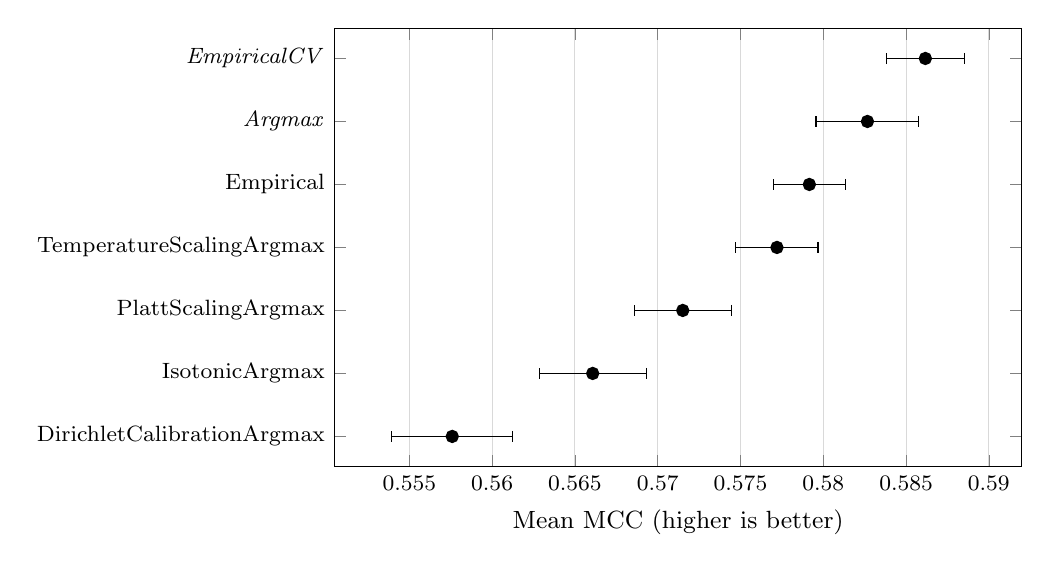
\begin{tikzpicture}
\begin{axis}[
    width=0.85\textwidth, height=7.15cm,
    xlabel={Mean MCC (higher is better)},
    symbolic y coords={{EmpiricalCV},{Argmax},{Empirical},{TemperatureScalingArgmax},{PlattScalingArgmax},{IsotonicArgmax},{DirichletCalibrationArgmax}},
    ytick={{EmpiricalCV},{Argmax},{Empirical},{TemperatureScalingArgmax},{PlattScalingArgmax},{IsotonicArgmax},{DirichletCalibrationArgmax}},
    yticklabels={\textit{EmpiricalCV},\textit{Argmax},Empirical,TemperatureScalingArgmax,PlattScalingArgmax,IsotonicArgmax,DirichletCalibrationArgmax},
    y dir=reverse,
    enlarge y limits=0.08,
    xmajorgrids=true,
    major grid style={draw=black!15, line width=0.3pt},
    scaled x ticks=false,
    xticklabel style={/pgf/number format/fixed, /pgf/number format/precision=3},
    tick label style={font=\footnotesize},
    label style={font=\small},
    every axis plot/.append style={thick},
]
\addplot[only marks, mark=*, mark size=2pt, color=black, error bars/x dir=both, error bars/x explicit, error bars/error bar style={color=black, line width=0.5pt}] coordinates { (0.586167,{EmpiricalCV}) +- (0.00235058,0) };
\addplot[only marks, mark=*, mark size=2pt, color=black, error bars/x dir=both, error bars/x explicit, error bars/error bar style={color=black, line width=0.5pt}] coordinates { (0.582668,{Argmax}) +- (0.00310402,0) };
\addplot[only marks, mark=*, mark size=2pt, color=black, error bars/x dir=both, error bars/x explicit, error bars/error bar style={color=black, line width=0.5pt}] coordinates { (0.57916,{Empirical}) +- (0.00218688,0) };
\addplot[only marks, mark=*, mark size=2pt, color=black, error bars/x dir=both, error bars/x explicit, error bars/error bar style={color=black, line width=0.5pt}] coordinates { (0.577204,{TemperatureScalingArgmax}) +- (0.00247722,0) };
\addplot[only marks, mark=*, mark size=2pt, color=black, error bars/x dir=both, error bars/x explicit, error bars/error bar style={color=black, line width=0.5pt}] coordinates { (0.571515,{PlattScalingArgmax}) +- (0.00292098,0) };
\addplot[only marks, mark=*, mark size=2pt, color=black, error bars/x dir=both, error bars/x explicit, error bars/error bar style={color=black, line width=0.5pt}] coordinates { (0.566076,{IsotonicArgmax}) +- (0.00322504,0) };
\addplot[only marks, mark=*, mark size=2pt, color=black, error bars/x dir=both, error bars/x explicit, error bars/error bar style={color=black, line width=0.5pt}] coordinates { (0.557592,{DirichletCalibrationArgmax}) +- (0.00365129,0) };
\end{axis}
\end{tikzpicture}%
}
\caption{adult: MCC on TabM (higher is better). Each dot is a strategy's mean over ten seeds with a $\pm 1$ SE horizontal bar; rows are sorted by mean, and the best strategy and any whose interval overlaps it are italicized.}%
\label{fig:ci-adult-mcc}
\end{figure}


Figures~\ref{fig:win-counts-binary-cost} and~\ref{fig:win-counts-binary-max} give the per-strategy win and tie rates under the $\pm 1$ SE overlap rule, broken out by base classifier and by dataset size and imbalance bucket; the figure captions document the reading convention and the bootstrap half-width.

% Auto-generated by experiments.analysis.generate_win_counts --- do not edit.
\begin{figure}[H]
\centering
\adjustbox{max width=\textwidth}{%
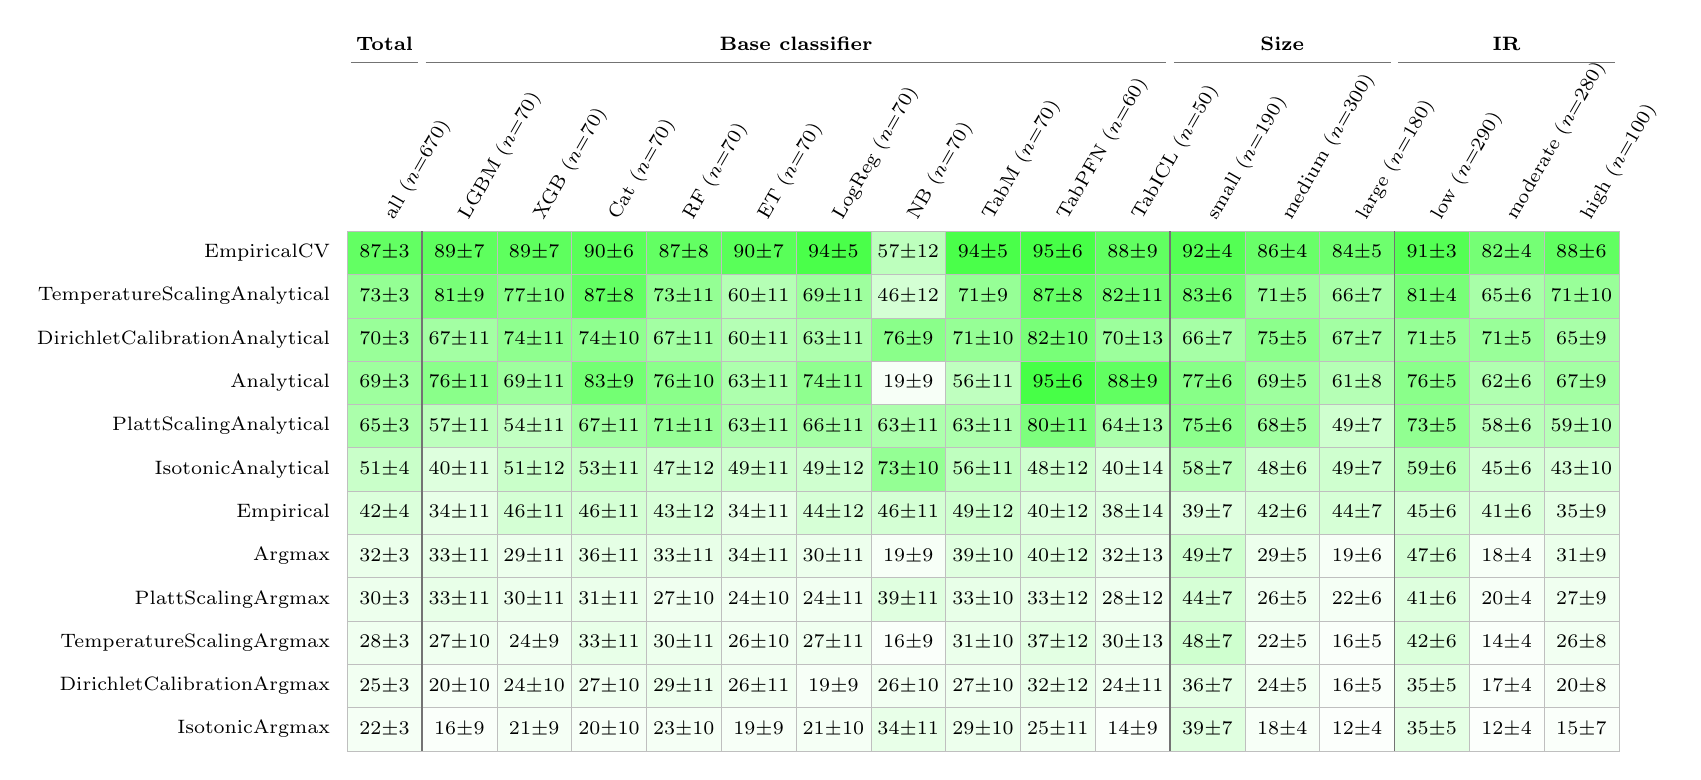
\begin{tikzpicture}[
    x=0.95cm, y=0.55cm,
    cell/.style={rectangle, draw=black!25, line width=0.2pt,
        minimum width=0.95cm, minimum height=0.55cm,
        anchor=center, font=\scriptsize, inner sep=0pt},
    rowlbl/.style={font=\scriptsize, anchor=east},
    collbl/.style={font=\scriptsize, anchor=west, rotate=60},
    grouplbl/.style={font=\scriptsize\bfseries, anchor=south},
    sep/.style={draw=black!55, line width=0.5pt},
]
\node[cell, fill=green!61] at (1, 12) {$87{\pm}3$};
\node[cell, fill=green!63] at (2, 12) {$89{\pm}7$};
\node[cell, fill=green!63] at (3, 12) {$89{\pm}7$};
\node[cell, fill=green!65] at (4, 12) {$90{\pm}6$};
\node[cell, fill=green!61] at (5, 12) {$87{\pm}8$};
\node[cell, fill=green!65] at (6, 12) {$90{\pm}7$};
\node[cell, fill=green!71] at (7, 12) {$94{\pm}5$};
\node[cell, fill=green!26] at (8, 12) {$57{\pm}12$};
\node[cell, fill=green!71] at (9, 12) {$94{\pm}5$};
\node[cell, fill=green!72] at (10, 12) {$95{\pm}6$};
\node[cell, fill=green!62] at (11, 12) {$88{\pm}9$};
\node[cell, fill=green!67] at (12, 12) {$92{\pm}4$};
\node[cell, fill=green!59] at (13, 12) {$86{\pm}4$};
\node[cell, fill=green!57] at (14, 12) {$84{\pm}5$};
\node[cell, fill=green!67] at (15, 12) {$91{\pm}3$};
\node[cell, fill=green!54] at (16, 12) {$82{\pm}4$};
\node[cell, fill=green!62] at (17, 12) {$88{\pm}6$};
\node[cell, fill=green!42] at (1, 11) {$73{\pm}3$};
\node[cell, fill=green!53] at (2, 11) {$81{\pm}9$};
\node[cell, fill=green!48] at (3, 11) {$77{\pm}10$};
\node[cell, fill=green!61] at (4, 11) {$87{\pm}8$};
\node[cell, fill=green!42] at (5, 11) {$73{\pm}11$};
\node[cell, fill=green!29] at (6, 11) {$60{\pm}11$};
\node[cell, fill=green!38] at (7, 11) {$69{\pm}11$};
\node[cell, fill=green!17] at (8, 11) {$46{\pm}12$};
\node[cell, fill=green!41] at (9, 11) {$71{\pm}9$};
\node[cell, fill=green!60] at (10, 11) {$87{\pm}8$};
\node[cell, fill=green!54] at (11, 11) {$82{\pm}11$};
\node[cell, fill=green!55] at (12, 11) {$83{\pm}6$};
\node[cell, fill=green!40] at (13, 11) {$71{\pm}5$};
\node[cell, fill=green!34] at (14, 11) {$66{\pm}7$};
\node[cell, fill=green!53] at (15, 11) {$81{\pm}4$};
\node[cell, fill=green!34] at (16, 11) {$65{\pm}6$};
\node[cell, fill=green!40] at (17, 11) {$71{\pm}10$};
\node[cell, fill=green!40] at (1, 10) {$70{\pm}3$};
\node[cell, fill=green!36] at (2, 10) {$67{\pm}11$};
\node[cell, fill=green!44] at (3, 10) {$74{\pm}11$};
\node[cell, fill=green!44] at (4, 10) {$74{\pm}10$};
\node[cell, fill=green!36] at (5, 10) {$67{\pm}11$};
\node[cell, fill=green!29] at (6, 10) {$60{\pm}11$};
\node[cell, fill=green!32] at (7, 10) {$63{\pm}11$};
\node[cell, fill=green!46] at (8, 10) {$76{\pm}9$};
\node[cell, fill=green!41] at (9, 10) {$71{\pm}10$};
\node[cell, fill=green!53] at (10, 10) {$82{\pm}10$};
\node[cell, fill=green!39] at (11, 10) {$70{\pm}13$};
\node[cell, fill=green!35] at (12, 10) {$66{\pm}7$};
\node[cell, fill=green!45] at (13, 10) {$75{\pm}5$};
\node[cell, fill=green!36] at (14, 10) {$67{\pm}7$};
\node[cell, fill=green!41] at (15, 10) {$71{\pm}5$};
\node[cell, fill=green!40] at (16, 10) {$71{\pm}5$};
\node[cell, fill=green!34] at (17, 10) {$65{\pm}9$};
\node[cell, fill=green!38] at (1, 9) {$69{\pm}3$};
\node[cell, fill=green!46] at (2, 9) {$76{\pm}11$};
\node[cell, fill=green!38] at (3, 9) {$69{\pm}11$};
\node[cell, fill=green!55] at (4, 9) {$83{\pm}9$};
\node[cell, fill=green!46] at (5, 9) {$76{\pm}10$};
\node[cell, fill=green!32] at (6, 9) {$63{\pm}11$};
\node[cell, fill=green!44] at (7, 9) {$74{\pm}11$};
\node[cell, fill=green!3] at (8, 9) {$19{\pm}9$};
\node[cell, fill=green!25] at (9, 9) {$56{\pm}11$};
\node[cell, fill=green!72] at (10, 9) {$95{\pm}6$};
\node[cell, fill=green!62] at (11, 9) {$88{\pm}9$};
\node[cell, fill=green!47] at (12, 9) {$77{\pm}6$};
\node[cell, fill=green!38] at (13, 9) {$69{\pm}5$};
\node[cell, fill=green!29] at (14, 9) {$61{\pm}8$};
\node[cell, fill=green!46] at (15, 9) {$76{\pm}5$};
\node[cell, fill=green!31] at (16, 9) {$62{\pm}6$};
\node[cell, fill=green!36] at (17, 9) {$67{\pm}9$};
\node[cell, fill=green!33] at (1, 8) {$65{\pm}3$};
\node[cell, fill=green!26] at (2, 8) {$57{\pm}11$};
\node[cell, fill=green!24] at (3, 8) {$54{\pm}11$};
\node[cell, fill=green!36] at (4, 8) {$67{\pm}11$};
\node[cell, fill=green!41] at (5, 8) {$71{\pm}11$};
\node[cell, fill=green!32] at (6, 8) {$63{\pm}11$};
\node[cell, fill=green!35] at (7, 8) {$66{\pm}11$};
\node[cell, fill=green!32] at (8, 8) {$63{\pm}11$};
\node[cell, fill=green!32] at (9, 8) {$63{\pm}11$};
\node[cell, fill=green!51] at (10, 8) {$80{\pm}11$};
\node[cell, fill=green!33] at (11, 8) {$64{\pm}13$};
\node[cell, fill=green!45] at (12, 8) {$75{\pm}6$};
\node[cell, fill=green!37] at (13, 8) {$68{\pm}5$};
\node[cell, fill=green!19] at (14, 8) {$49{\pm}7$};
\node[cell, fill=green!43] at (15, 8) {$73{\pm}5$};
\node[cell, fill=green!27] at (16, 8) {$58{\pm}6$};
\node[cell, fill=green!28] at (17, 8) {$59{\pm}10$};
\node[cell, fill=green!21] at (1, 7) {$51{\pm}4$};
\node[cell, fill=green!13] at (2, 7) {$40{\pm}11$};
\node[cell, fill=green!21] at (3, 7) {$51{\pm}12$};
\node[cell, fill=green!22] at (4, 7) {$53{\pm}11$};
\node[cell, fill=green!18] at (5, 7) {$47{\pm}12$};
\node[cell, fill=green!19] at (6, 7) {$49{\pm}11$};
\node[cell, fill=green!19] at (7, 7) {$49{\pm}12$};
\node[cell, fill=green!42] at (8, 7) {$73{\pm}10$};
\node[cell, fill=green!25] at (9, 7) {$56{\pm}11$};
\node[cell, fill=green!19] at (10, 7) {$48{\pm}12$};
\node[cell, fill=green!13] at (11, 7) {$40{\pm}14$};
\node[cell, fill=green!27] at (12, 7) {$58{\pm}7$};
\node[cell, fill=green!18] at (13, 7) {$48{\pm}6$};
\node[cell, fill=green!19] at (14, 7) {$49{\pm}7$};
\node[cell, fill=green!28] at (15, 7) {$59{\pm}6$};
\node[cell, fill=green!16] at (16, 7) {$45{\pm}6$};
\node[cell, fill=green!15] at (17, 7) {$43{\pm}10$};
\node[cell, fill=green!14] at (1, 6) {$42{\pm}4$};
\node[cell, fill=green!9] at (2, 6) {$34{\pm}11$};
\node[cell, fill=green!17] at (3, 6) {$46{\pm}11$};
\node[cell, fill=green!17] at (4, 6) {$46{\pm}11$};
\node[cell, fill=green!15] at (5, 6) {$43{\pm}12$};
\node[cell, fill=green!9] at (6, 6) {$34{\pm}11$};
\node[cell, fill=green!16] at (7, 6) {$44{\pm}12$};
\node[cell, fill=green!17] at (8, 6) {$46{\pm}11$};
\node[cell, fill=green!19] at (9, 6) {$49{\pm}12$};
\node[cell, fill=green!13] at (10, 6) {$40{\pm}12$};
\node[cell, fill=green!12] at (11, 6) {$38{\pm}14$};
\node[cell, fill=green!12] at (12, 6) {$39{\pm}7$};
\node[cell, fill=green!14] at (13, 6) {$42{\pm}6$};
\node[cell, fill=green!16] at (14, 6) {$44{\pm}7$};
\node[cell, fill=green!16] at (15, 6) {$45{\pm}6$};
\node[cell, fill=green!14] at (16, 6) {$41{\pm}6$};
\node[cell, fill=green!10] at (17, 6) {$35{\pm}9$};
\node[cell, fill=green!8] at (1, 5) {$32{\pm}3$};
\node[cell, fill=green!9] at (2, 5) {$33{\pm}11$};
\node[cell, fill=green!7] at (3, 5) {$29{\pm}11$};
\node[cell, fill=green!10] at (4, 5) {$36{\pm}11$};
\node[cell, fill=green!9] at (5, 5) {$33{\pm}11$};
\node[cell, fill=green!9] at (6, 5) {$34{\pm}11$};
\node[cell, fill=green!7] at (7, 5) {$30{\pm}11$};
\node[cell, fill=green!3] at (8, 5) {$19{\pm}9$};
\node[cell, fill=green!12] at (9, 5) {$39{\pm}10$};
\node[cell, fill=green!13] at (10, 5) {$40{\pm}12$};
\node[cell, fill=green!8] at (11, 5) {$32{\pm}13$};
\node[cell, fill=green!19] at (12, 5) {$49{\pm}7$};
\node[cell, fill=green!7] at (13, 5) {$29{\pm}5$};
\node[cell, fill=green!3] at (14, 5) {$19{\pm}6$};
\node[cell, fill=green!17] at (15, 5) {$47{\pm}6$};
\node[cell, fill=green!3] at (16, 5) {$18{\pm}4$};
\node[cell, fill=green!8] at (17, 5) {$31{\pm}9$};
\node[cell, fill=green!7] at (1, 4) {$30{\pm}3$};
\node[cell, fill=green!9] at (2, 4) {$33{\pm}11$};
\node[cell, fill=green!7] at (3, 4) {$30{\pm}11$};
\node[cell, fill=green!8] at (4, 4) {$31{\pm}11$};
\node[cell, fill=green!6] at (5, 4) {$27{\pm}10$};
\node[cell, fill=green!5] at (6, 4) {$24{\pm}10$};
\node[cell, fill=green!5] at (7, 4) {$24{\pm}11$};
\node[cell, fill=green!12] at (8, 4) {$39{\pm}11$};
\node[cell, fill=green!9] at (9, 4) {$33{\pm}10$};
\node[cell, fill=green!9] at (10, 4) {$33{\pm}12$};
\node[cell, fill=green!6] at (11, 4) {$28{\pm}12$};
\node[cell, fill=green!16] at (12, 4) {$44{\pm}7$};
\node[cell, fill=green!6] at (13, 4) {$26{\pm}5$};
\node[cell, fill=green!4] at (14, 4) {$22{\pm}6$};
\node[cell, fill=green!13] at (15, 4) {$41{\pm}6$};
\node[cell, fill=green!3] at (16, 4) {$20{\pm}4$};
\node[cell, fill=green!6] at (17, 4) {$27{\pm}9$};
\node[cell, fill=green!6] at (1, 3) {$28{\pm}3$};
\node[cell, fill=green!6] at (2, 3) {$27{\pm}10$};
\node[cell, fill=green!5] at (3, 3) {$24{\pm}9$};
\node[cell, fill=green!9] at (4, 3) {$33{\pm}11$};
\node[cell, fill=green!7] at (5, 3) {$30{\pm}11$};
\node[cell, fill=green!5] at (6, 3) {$26{\pm}10$};
\node[cell, fill=green!6] at (7, 3) {$27{\pm}11$};
\node[cell, fill=green!2] at (8, 3) {$16{\pm}9$};
\node[cell, fill=green!8] at (9, 3) {$31{\pm}10$};
\node[cell, fill=green!11] at (10, 3) {$37{\pm}12$};
\node[cell, fill=green!7] at (11, 3) {$30{\pm}13$};
\node[cell, fill=green!19] at (12, 3) {$48{\pm}7$};
\node[cell, fill=green!4] at (13, 3) {$22{\pm}5$};
\node[cell, fill=green!2] at (14, 3) {$16{\pm}5$};
\node[cell, fill=green!14] at (15, 3) {$42{\pm}6$};
\node[cell, fill=green!2] at (16, 3) {$14{\pm}4$};
\node[cell, fill=green!5] at (17, 3) {$26{\pm}8$};
\node[cell, fill=green!5] at (1, 2) {$25{\pm}3$};
\node[cell, fill=green!3] at (2, 2) {$20{\pm}10$};
\node[cell, fill=green!5] at (3, 2) {$24{\pm}10$};
\node[cell, fill=green!6] at (4, 2) {$27{\pm}10$};
\node[cell, fill=green!7] at (5, 2) {$29{\pm}11$};
\node[cell, fill=green!5] at (6, 2) {$26{\pm}11$};
\node[cell, fill=green!3] at (7, 2) {$19{\pm}9$};
\node[cell, fill=green!5] at (8, 2) {$26{\pm}10$};
\node[cell, fill=green!6] at (9, 2) {$27{\pm}10$};
\node[cell, fill=green!8] at (10, 2) {$32{\pm}12$};
\node[cell, fill=green!5] at (11, 2) {$24{\pm}11$};
\node[cell, fill=green!10] at (12, 2) {$36{\pm}7$};
\node[cell, fill=green!5] at (13, 2) {$24{\pm}5$};
\node[cell, fill=green!2] at (14, 2) {$16{\pm}5$};
\node[cell, fill=green!10] at (15, 2) {$35{\pm}5$};
\node[cell, fill=green!2] at (16, 2) {$17{\pm}4$};
\node[cell, fill=green!3] at (17, 2) {$20{\pm}8$};
\node[cell, fill=green!4] at (1, 1) {$22{\pm}3$};
\node[cell, fill=green!2] at (2, 1) {$16{\pm}9$};
\node[cell, fill=green!4] at (3, 1) {$21{\pm}9$};
\node[cell, fill=green!3] at (4, 1) {$20{\pm}10$};
\node[cell, fill=green!4] at (5, 1) {$23{\pm}10$};
\node[cell, fill=green!3] at (6, 1) {$19{\pm}9$};
\node[cell, fill=green!4] at (7, 1) {$21{\pm}10$};
\node[cell, fill=green!9] at (8, 1) {$34{\pm}11$};
\node[cell, fill=green!7] at (9, 1) {$29{\pm}10$};
\node[cell, fill=green!5] at (10, 1) {$25{\pm}11$};
\node[cell, fill=green!2] at (11, 1) {$14{\pm}9$};
\node[cell, fill=green!12] at (12, 1) {$39{\pm}7$};
\node[cell, fill=green!3] at (13, 1) {$18{\pm}4$};
\node[cell, fill=green!1] at (14, 1) {$12{\pm}4$};
\node[cell, fill=green!10] at (15, 1) {$35{\pm}5$};
\node[cell, fill=green!1] at (16, 1) {$12{\pm}4$};
\node[cell, fill=green!2] at (17, 1) {$15{\pm}7$};
\node[rowlbl] at (0.4, 12) {EmpiricalCV};
\node[rowlbl] at (0.4, 11) {TemperatureScalingAnalytical};
\node[rowlbl] at (0.4, 10) {DirichletCalibrationAnalytical};
\node[rowlbl] at (0.4, 9) {Analytical};
\node[rowlbl] at (0.4, 8) {PlattScalingAnalytical};
\node[rowlbl] at (0.4, 7) {IsotonicAnalytical};
\node[rowlbl] at (0.4, 6) {Empirical};
\node[rowlbl] at (0.4, 5) {Argmax};
\node[rowlbl] at (0.4, 4) {PlattScalingArgmax};
\node[rowlbl] at (0.4, 3) {TemperatureScalingArgmax};
\node[rowlbl] at (0.4, 2) {DirichletCalibrationArgmax};
\node[rowlbl] at (0.4, 1) {IsotonicArgmax};
\node[collbl] at (1, 12.6) {all ($n{=}670$)};
\node[collbl] at (2, 12.6) {LGBM ($n{=}70$)};
\node[collbl] at (3, 12.6) {XGB ($n{=}70$)};
\node[collbl] at (4, 12.6) {Cat ($n{=}70$)};
\node[collbl] at (5, 12.6) {RF ($n{=}70$)};
\node[collbl] at (6, 12.6) {ET ($n{=}70$)};
\node[collbl] at (7, 12.6) {LogReg ($n{=}70$)};
\node[collbl] at (8, 12.6) {NB ($n{=}70$)};
\node[collbl] at (9, 12.6) {TabM ($n{=}70$)};
\node[collbl] at (10, 12.6) {TabPFN ($n{=}60$)};
\node[collbl] at (11, 12.6) {TabICL ($n{=}50$)};
\node[collbl] at (12, 12.6) {small ($n{=}190$)};
\node[collbl] at (13, 12.6) {medium ($n{=}300$)};
\node[collbl] at (14, 12.6) {large ($n{=}180$)};
\node[collbl] at (15, 12.6) {low ($n{=}290$)};
\node[collbl] at (16, 12.6) {moderate ($n{=}280$)};
\node[collbl] at (17, 12.6) {high ($n{=}100$)};
\draw[black!55, line width=0.5pt] (0.55, 16.4) -- (1.45, 16.4);
\node[grouplbl] at (1.0, 16.45) {Total};
\draw[black!55, line width=0.5pt] (1.55, 16.4) -- (11.45, 16.4);
\node[grouplbl] at (6.5, 16.45) {Base classifier};
\draw[black!55, line width=0.5pt] (11.55, 16.4) -- (14.45, 16.4);
\node[grouplbl] at (13.0, 16.45) {Size};
\draw[black!55, line width=0.5pt] (14.55, 16.4) -- (17.45, 16.4);
\node[grouplbl] at (16.0, 16.45) {IR};
\draw[sep] (1.5, 0.5) -- (1.5, 12.5);
\draw[sep] (11.5, 0.5) -- (11.5, 12.5);
\draw[sep] (14.5, 0.5) -- (14.5, 12.5);
\end{tikzpicture}%
}
\caption{Per-strategy win/tie rates on binary cost-matrix objectives. Each cell reads ``$r{\pm}H$'': $r$ is the percentage of (dataset, model, objective) cells in the slice where the strategy won or tied the per-row best under the $\pm 1$ SE overlap rule, and $H$ is the half-width of a 95\% cluster-bootstrap confidence interval for $r$ (percentage points). Shading is a quadratic ($\mathrm{rate}^2$) scale of $r$. Strategies are sorted by overall win rate; ``$n$'' under each column header is the maximum applicable cell count for that slice.}%
\label{fig:win-counts-binary-cost}
\end{figure}


% Auto-generated by experiments.analysis.generate_win_counts --- do not edit.
\begin{figure}[H]
\centering
\adjustbox{max width=\textwidth}{%
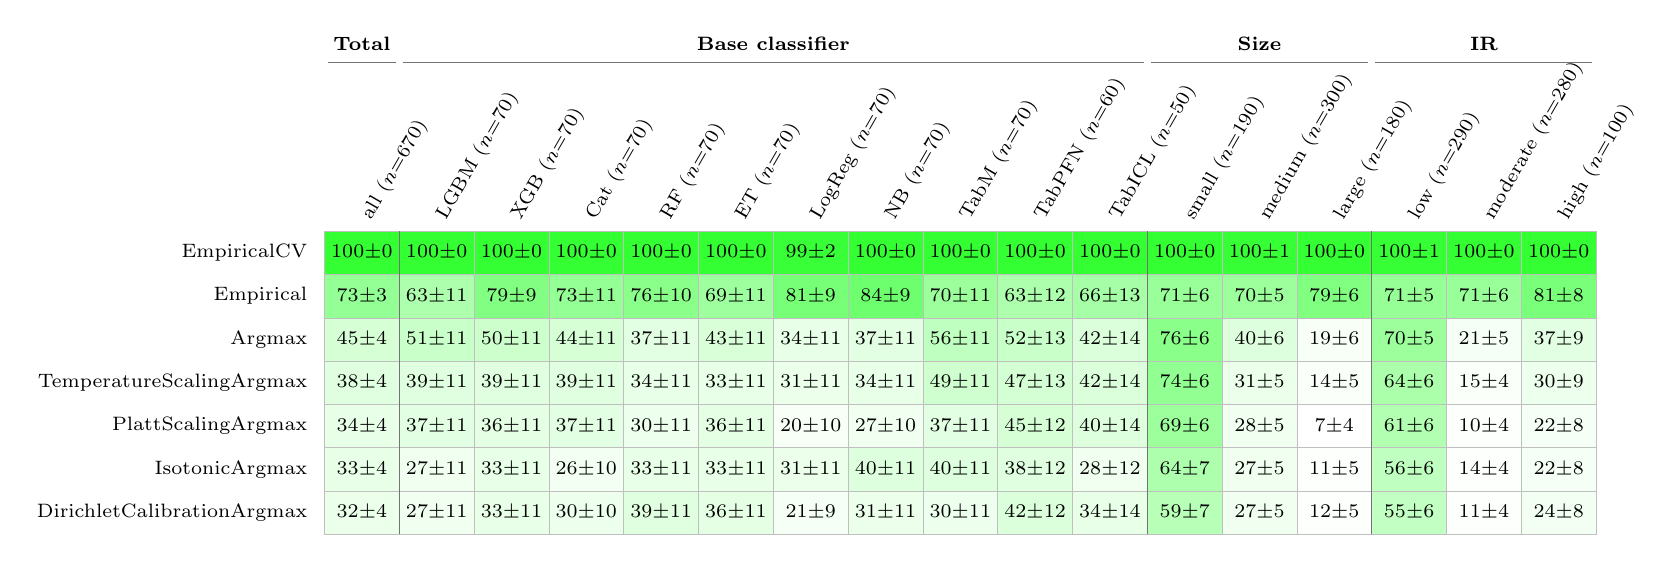
\begin{tikzpicture}[
    x=0.95cm, y=0.55cm,
    cell/.style={rectangle, draw=black!25, line width=0.2pt,
        minimum width=0.95cm, minimum height=0.55cm,
        anchor=center, font=\scriptsize, inner sep=0pt},
    rowlbl/.style={font=\scriptsize, anchor=east},
    collbl/.style={font=\scriptsize, anchor=west, rotate=60},
    grouplbl/.style={font=\scriptsize\bfseries, anchor=south},
    sep/.style={draw=black!55, line width=0.5pt},
]
\node[cell, fill=green!80] at (1, 7) {$100{\pm}0$};
\node[cell, fill=green!80] at (2, 7) {$100{\pm}0$};
\node[cell, fill=green!80] at (3, 7) {$100{\pm}0$};
\node[cell, fill=green!80] at (4, 7) {$100{\pm}0$};
\node[cell, fill=green!80] at (5, 7) {$100{\pm}0$};
\node[cell, fill=green!80] at (6, 7) {$100{\pm}0$};
\node[cell, fill=green!78] at (7, 7) {$99{\pm}2$};
\node[cell, fill=green!80] at (8, 7) {$100{\pm}0$};
\node[cell, fill=green!80] at (9, 7) {$100{\pm}0$};
\node[cell, fill=green!80] at (10, 7) {$100{\pm}0$};
\node[cell, fill=green!80] at (11, 7) {$100{\pm}0$};
\node[cell, fill=green!80] at (12, 7) {$100{\pm}0$};
\node[cell, fill=green!79] at (13, 7) {$100{\pm}1$};
\node[cell, fill=green!80] at (14, 7) {$100{\pm}0$};
\node[cell, fill=green!79] at (15, 7) {$100{\pm}1$};
\node[cell, fill=green!80] at (16, 7) {$100{\pm}0$};
\node[cell, fill=green!80] at (17, 7) {$100{\pm}0$};
\node[cell, fill=green!42] at (1, 6) {$73{\pm}3$};
\node[cell, fill=green!32] at (2, 6) {$63{\pm}11$};
\node[cell, fill=green!49] at (3, 6) {$79{\pm}9$};
\node[cell, fill=green!42] at (4, 6) {$73{\pm}11$};
\node[cell, fill=green!46] at (5, 6) {$76{\pm}10$};
\node[cell, fill=green!38] at (6, 6) {$69{\pm}11$};
\node[cell, fill=green!53] at (7, 6) {$81{\pm}9$};
\node[cell, fill=green!57] at (8, 6) {$84{\pm}9$};
\node[cell, fill=green!39] at (9, 6) {$70{\pm}11$};
\node[cell, fill=green!32] at (10, 6) {$63{\pm}12$};
\node[cell, fill=green!35] at (11, 6) {$66{\pm}13$};
\node[cell, fill=green!40] at (12, 6) {$71{\pm}6$};
\node[cell, fill=green!39] at (13, 6) {$70{\pm}5$};
\node[cell, fill=green!50] at (14, 6) {$79{\pm}6$};
\node[cell, fill=green!41] at (15, 6) {$71{\pm}5$};
\node[cell, fill=green!40] at (16, 6) {$71{\pm}6$};
\node[cell, fill=green!52] at (17, 6) {$81{\pm}8$};
\node[cell, fill=green!16] at (1, 5) {$45{\pm}4$};
\node[cell, fill=green!21] at (2, 5) {$51{\pm}11$};
\node[cell, fill=green!20] at (3, 5) {$50{\pm}11$};
\node[cell, fill=green!16] at (4, 5) {$44{\pm}11$};
\node[cell, fill=green!11] at (5, 5) {$37{\pm}11$};
\node[cell, fill=green!15] at (6, 5) {$43{\pm}11$};
\node[cell, fill=green!9] at (7, 5) {$34{\pm}11$};
\node[cell, fill=green!11] at (8, 5) {$37{\pm}11$};
\node[cell, fill=green!25] at (9, 5) {$56{\pm}11$};
\node[cell, fill=green!21] at (10, 5) {$52{\pm}13$};
\node[cell, fill=green!14] at (11, 5) {$42{\pm}14$};
\node[cell, fill=green!46] at (12, 5) {$76{\pm}6$};
\node[cell, fill=green!13] at (13, 5) {$40{\pm}6$};
\node[cell, fill=green!3] at (14, 5) {$19{\pm}6$};
\node[cell, fill=green!39] at (15, 5) {$70{\pm}5$};
\node[cell, fill=green!4] at (16, 5) {$21{\pm}5$};
\node[cell, fill=green!11] at (17, 5) {$37{\pm}9$};
\node[cell, fill=green!12] at (1, 4) {$38{\pm}4$};
\node[cell, fill=green!12] at (2, 4) {$39{\pm}11$};
\node[cell, fill=green!12] at (3, 4) {$39{\pm}11$};
\node[cell, fill=green!12] at (4, 4) {$39{\pm}11$};
\node[cell, fill=green!9] at (5, 4) {$34{\pm}11$};
\node[cell, fill=green!9] at (6, 4) {$33{\pm}11$};
\node[cell, fill=green!8] at (7, 4) {$31{\pm}11$};
\node[cell, fill=green!9] at (8, 4) {$34{\pm}11$};
\node[cell, fill=green!19] at (9, 4) {$49{\pm}11$};
\node[cell, fill=green!17] at (10, 4) {$47{\pm}13$};
\node[cell, fill=green!14] at (11, 4) {$42{\pm}14$};
\node[cell, fill=green!43] at (12, 4) {$74{\pm}6$};
\node[cell, fill=green!8] at (13, 4) {$31{\pm}5$};
\node[cell, fill=green!2] at (14, 4) {$14{\pm}5$};
\node[cell, fill=green!33] at (15, 4) {$64{\pm}6$};
\node[cell, fill=green!2] at (16, 4) {$15{\pm}4$};
\node[cell, fill=green!7] at (17, 4) {$30{\pm}9$};
\node[cell, fill=green!9] at (1, 3) {$34{\pm}4$};
\node[cell, fill=green!11] at (2, 3) {$37{\pm}11$};
\node[cell, fill=green!10] at (3, 3) {$36{\pm}11$};
\node[cell, fill=green!11] at (4, 3) {$37{\pm}11$};
\node[cell, fill=green!7] at (5, 3) {$30{\pm}11$};
\node[cell, fill=green!10] at (6, 3) {$36{\pm}11$};
\node[cell, fill=green!3] at (7, 3) {$20{\pm}10$};
\node[cell, fill=green!6] at (8, 3) {$27{\pm}10$};
\node[cell, fill=green!11] at (9, 3) {$37{\pm}11$};
\node[cell, fill=green!16] at (10, 3) {$45{\pm}12$};
\node[cell, fill=green!13] at (11, 3) {$40{\pm}14$};
\node[cell, fill=green!39] at (12, 3) {$69{\pm}6$};
\node[cell, fill=green!6] at (13, 3) {$28{\pm}5$};
\node[cell, fill=green!0] at (14, 3) {$7{\pm}4$};
\node[cell, fill=green!30] at (15, 3) {$61{\pm}6$};
\node[cell, fill=green!1] at (16, 3) {$10{\pm}4$};
\node[cell, fill=green!4] at (17, 3) {$22{\pm}8$};
\node[cell, fill=green!9] at (1, 2) {$33{\pm}4$};
\node[cell, fill=green!6] at (2, 2) {$27{\pm}11$};
\node[cell, fill=green!9] at (3, 2) {$33{\pm}11$};
\node[cell, fill=green!5] at (4, 2) {$26{\pm}10$};
\node[cell, fill=green!9] at (5, 2) {$33{\pm}11$};
\node[cell, fill=green!9] at (6, 2) {$33{\pm}11$};
\node[cell, fill=green!8] at (7, 2) {$31{\pm}11$};
\node[cell, fill=green!13] at (8, 2) {$40{\pm}11$};
\node[cell, fill=green!13] at (9, 2) {$40{\pm}11$};
\node[cell, fill=green!12] at (10, 2) {$38{\pm}12$};
\node[cell, fill=green!6] at (11, 2) {$28{\pm}12$};
\node[cell, fill=green!32] at (12, 2) {$64{\pm}7$};
\node[cell, fill=green!6] at (13, 2) {$27{\pm}5$};
\node[cell, fill=green!1] at (14, 2) {$11{\pm}5$};
\node[cell, fill=green!25] at (15, 2) {$56{\pm}6$};
\node[cell, fill=green!1] at (16, 2) {$14{\pm}4$};
\node[cell, fill=green!4] at (17, 2) {$22{\pm}8$};
\node[cell, fill=green!8] at (1, 1) {$32{\pm}4$};
\node[cell, fill=green!6] at (2, 1) {$27{\pm}11$};
\node[cell, fill=green!9] at (3, 1) {$33{\pm}11$};
\node[cell, fill=green!7] at (4, 1) {$30{\pm}10$};
\node[cell, fill=green!12] at (5, 1) {$39{\pm}11$};
\node[cell, fill=green!10] at (6, 1) {$36{\pm}11$};
\node[cell, fill=green!4] at (7, 1) {$21{\pm}9$};
\node[cell, fill=green!8] at (8, 1) {$31{\pm}11$};
\node[cell, fill=green!7] at (9, 1) {$30{\pm}11$};
\node[cell, fill=green!14] at (10, 1) {$42{\pm}12$};
\node[cell, fill=green!9] at (11, 1) {$34{\pm}14$};
\node[cell, fill=green!28] at (12, 1) {$59{\pm}7$};
\node[cell, fill=green!6] at (13, 1) {$27{\pm}5$};
\node[cell, fill=green!1] at (14, 1) {$12{\pm}5$};
\node[cell, fill=green!24] at (15, 1) {$55{\pm}6$};
\node[cell, fill=green!1] at (16, 1) {$11{\pm}4$};
\node[cell, fill=green!5] at (17, 1) {$24{\pm}8$};
\node[rowlbl] at (0.4, 7) {EmpiricalCV};
\node[rowlbl] at (0.4, 6) {Empirical};
\node[rowlbl] at (0.4, 5) {Argmax};
\node[rowlbl] at (0.4, 4) {TemperatureScalingArgmax};
\node[rowlbl] at (0.4, 3) {PlattScalingArgmax};
\node[rowlbl] at (0.4, 2) {IsotonicArgmax};
\node[rowlbl] at (0.4, 1) {DirichletCalibrationArgmax};
\node[collbl] at (1, 7.6) {all ($n{=}670$)};
\node[collbl] at (2, 7.6) {LGBM ($n{=}70$)};
\node[collbl] at (3, 7.6) {XGB ($n{=}70$)};
\node[collbl] at (4, 7.6) {Cat ($n{=}70$)};
\node[collbl] at (5, 7.6) {RF ($n{=}70$)};
\node[collbl] at (6, 7.6) {ET ($n{=}70$)};
\node[collbl] at (7, 7.6) {LogReg ($n{=}70$)};
\node[collbl] at (8, 7.6) {NB ($n{=}70$)};
\node[collbl] at (9, 7.6) {TabM ($n{=}70$)};
\node[collbl] at (10, 7.6) {TabPFN ($n{=}60$)};
\node[collbl] at (11, 7.6) {TabICL ($n{=}50$)};
\node[collbl] at (12, 7.6) {small ($n{=}190$)};
\node[collbl] at (13, 7.6) {medium ($n{=}300$)};
\node[collbl] at (14, 7.6) {large ($n{=}180$)};
\node[collbl] at (15, 7.6) {low ($n{=}290$)};
\node[collbl] at (16, 7.6) {moderate ($n{=}280$)};
\node[collbl] at (17, 7.6) {high ($n{=}100$)};
\draw[black!55, line width=0.5pt] (0.55, 11.4) -- (1.45, 11.4);
\node[grouplbl] at (1.0, 11.450000000000001) {Total};
\draw[black!55, line width=0.5pt] (1.55, 11.4) -- (11.45, 11.4);
\node[grouplbl] at (6.5, 11.450000000000001) {Base classifier};
\draw[black!55, line width=0.5pt] (11.55, 11.4) -- (14.45, 11.4);
\node[grouplbl] at (13.0, 11.450000000000001) {Size};
\draw[black!55, line width=0.5pt] (14.55, 11.4) -- (17.45, 11.4);
\node[grouplbl] at (16.0, 11.450000000000001) {IR};
\draw[sep] (1.5, 0.5) -- (1.5, 7.5);
\draw[sep] (11.5, 0.5) -- (11.5, 7.5);
\draw[sep] (14.5, 0.5) -- (14.5, 7.5);
\end{tikzpicture}%
}
\caption{Per-strategy win/tie rates on binary maximization metrics. Each cell reads ``$r{\pm}H$'': $r$ is the percentage of (dataset, model, objective) cells in the slice where the strategy won or tied the per-row best under the $\pm 1$ SE overlap rule, and $H$ is the half-width of a 95\% cluster-bootstrap confidence interval for $r$ (percentage points). Shading is a quadratic ($\mathrm{rate}^2$) scale of $r$. Strategies are sorted by overall win rate; ``$n$'' under each column header is the maximum applicable cell count for that slice.}%
\label{fig:win-counts-binary-max}
\end{figure}


\section{Summary of binary analysis}

The binary campaign shows an interaction between cost asymmetry and estimator calibration.

When the base estimator is well calibrated, as for the three deep tabular models here, the bare Analytical threshold is near-optimal under the decomposable cost objectives and consumes no held-out data.

When the estimator is miscalibrated, the analytical rule is far from optimal under heavy asymmetry, and the route back to competitive loss depends on the data budget available for tuning. A single $10\%$ validation split is too small to tune the threshold reliably under heavy asymmetry, so Empirical is in aggregate no better than the analytical plug-in. Cross-validation over the full pool makes EmpiricalCV the most reliable strategy across the campaign. For miscalibrated non-neural estimators specifically, post-hoc parametric calibration composed with the analytical rule is the lowest-loss option when the objective admits a closed-form optimum under calibrated probabilities.
